% Tizenharmadik előadás

\chapter{Az ARM szerver processzorok}

\section{Változások az adatközpontokban}
A hagyományos adatközpontok szerepe 2010 környékén megváltozott, mivel megjelentek a felhő számítási lehetőségek és az IoT.
Ekkor háromféle adatközpont alakult ki:
\begin{itemize}
    \item hiperskálázott adatközpontok
    \item hagyományos, nagyvállalati adatközpontok
    \item edge (perem) szerverek
\end{itemize}

\subsection{Hiperskálázott DC-k}
A hiperskálázott adatközpontok a dinamikusan változó igények kiszolgálására szolgálnak.
Ezek elég nagy adatközpontok, több tízezer szerverrel.
Különbséget lehet tenni Tier 1 és Tier 2 adatközpontok között, ahol a Tier 1-es központok a legnagyobb szolgáltatókat szolgálják ki (AWS, Google, Facebook), a Tier 2-esek pedig a nagy felhőszolgáltatókat, SaaS platformokat és közösségi oldalakat.

\subsection{Nagyvállalati adatközpontok}
A hagyományos adatközpontok állandóbb terhelést szolgálnak ki, kb. 1000 szerverig soroljuk ide a DC-ket.

\subsection{Edge (perem) szerverek}
Ezek egy közbülső réteget jelentenek az IoT eszközök és a cloud adatközpontok között.
Maga a fogalom körülbelül 10 éve jelent meg, az elosztott számításokkal együtt.
A peremszerverek az IoT eszközökhöz közel helyezkednek el, így gyorsan, kis válaszidővel tud számításokat végezni az IoT eszközök számára.

\section{Az ARM alapú szerverek kialakulása}
A processzorok lehetnek CISC és RISC architektúrájúak, az ARM RISC, az x86 pedig CISC.
A RISC egy load-store architektúra, ami azt jelenti, hogy az operandusok csak a regiszterekben lehetnek, azokat külön utasításokkal kell betölteni és visszatölteni a memóriába.
Az x86 processzorok ezzel szemben megengednek operandus betöltést a memóriából.
Ez a módszer egyszerűsíti a programozást, de a memóriacímzés miatt változó hosszú utasításokat kell használni, ami a dekódolást sokkal lassabbá teszi, valamint a memóriából történő adatlehívás is bonyolítja, lassítja a műveleteket.
A RISC-ek tehát kisebb teljesítmény igényűek.

A RISC-ek a 2000-es évek elején eltűntek a piacról, de a mobiloknál újra megjelentek és egyeduralkodóvá váltak.
Ezzel együtt a Caldexa cég elkezdett foglalkozni az ARM alapú szerverek fejlesztésével.
Azonban az ARMv7-et leváltotta a v8, így a Caldexa fejlesztései feleslegessé váltak, a cég csődbe ment.
Később az AMD is próbálkozott ARMv8 alapú processzorokkal, de az erre épülő szerver nem volt elég nagy teljesítményű.
Az Ampere cég fejlesztett még ARM alapú szerver processzorokkal, majd később megjelent a Qualcom, a Cavium és a Broadcom is szerver processzorokkal.

A fejlesztésnek volt még egy hulláma, amikor az ARM kihozta a v8.2 alapú Neoverse szerver processzor családját.
Az ARM ezzel a családdal egy nagyon dinamikus fejlesztést ígért, éves szinten 30\%-os gyorsulást.
Ez végül felül is múlták, az első generáció is 60\%-os javulást hozott.
A Neoverse mellett az Altra és a Graviton processzorok is piacképesek jelenleg, képesek felvenni a versenyt az AMD-vel és az Intellel is.
Ezek a processzorok a benchmarkok szerint jobb teljesítményt érnek el az Intellel szemben.

\section{Neoverse processzorok}
Az ARM Neoverse processzorok előnye a mobilokba szánt Cortex processzor.
A cél piac a nagy adatközpontoktól a peremszerverekig tart.

Érdekesség, hogy az ARM a szerver processzorai teljesítményét a Cosmos platformhoz képest adja meg, viszont a Cosmos családba tartozik a Cortex-A72 és a Cortex-A75 is, ahol az A72 v8, az A75 pedig v8.2 (így a teljesítményük is jelentősen eltér).

\subsection{Adatkapcsolat}
A Neoverse processzorok a gyűrűs adatkapcsolat helyett 2D mesh adatkapcsolati megoldást használnak, mivel több magnál ez hatékonyabb.

\subsection{Sorozatok}
A Neoverse család 3 sorozatból áll:
\begin{itemize}
    \item V: nagy teljesítmény
    \item N: jó teljesítmény/fogyasztás arány
    \item E: 5G eszközökre, routerekre, switchekre fejlesztve, kis fogyasztással
\end{itemize}
\begin{figure}[H]
    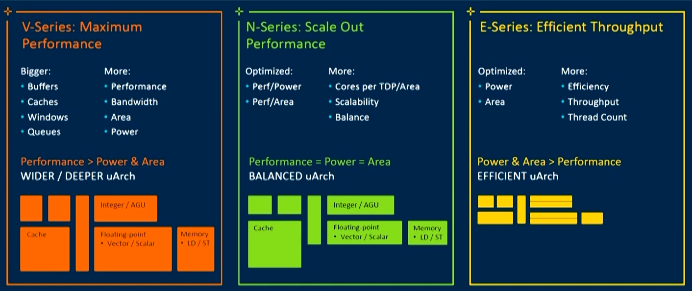
\includegraphics[width=0.8\textwidth]{sorozat}
    \centering
    \caption{Az ARM fejlesztési céljai sorozatok szerint}
    \label{fig:sorozat}
\end{figure}

\subsection{Támogatott új technológiák}
A Neoverse processzorok számos új technológiát támogatnak.

\subsubsection{DDR5}
A DDR5-ös memóriák 2020 végén jelentek meg, jellemzői:
\begin{itemize}
    \item kisebb feszültség (1.1V)
    \item magasabb átviteli ráta (DDR4 duplája)
    \item 2, egymástól független 32 bites memóriacsatornát alkalmaz
    \item a feszültségszabályzás az alaplaról a DIMM-re került
    \item a csatlakozófelülete nem változott
\end{itemize}
Csak kevés rendszer támogatja még, pl. Intel Alder Lake, AMD Zen 4.

\subsubsection{HBM - High Bandwidth Memory}
A nagy sávszélességű memóriák 2.5D tokozású memóriák, stack felépítéssel és nagyon széles adatinterfésszel (1024 bit).
Sávszélességük szintén nagyon nagy.
4 szeletből épülnek fel egy stack, egy processzorhoz négy szelet csatlakozik.

Egyik előnye, hogy kis energia szükséges egy átvitelhez.
2013-ban jelentek meg először, jelenleg a 2-es verziónál tart, de bejelentették a 3-asat is.

\subsubsection{PCIe 5.0}
A PCIe 5-ös verziója kb. megduplázta az előző verzió sebességét.
Már aktív használatban vannak.

\subsubsection{CCIX}
A CCIX (Cache Coherent Interconnect for Accelerators) egy nyílt szabvány, ami a gyorsítók összekapcsolására szolgál.
Ugyanazt a funkciót látja el, mint az Intel QuickPath Interconnect és az AMD Infinity Fabric.
A CCIX a heterogén rendszerekben teremt cache koherens kapcsolatot (pl. egy CPU és GPU között), így ez egy általánosan használható rendszerelem.

Átviteli protokoll szempontjából nem valósít meg teljesen új protokollt, hanem a CCIX 1.0 a PCIe 4.0-ra, a CCIX 1.1 pedig a PCIe 5.0-ra alapoz.

\subsubsection{CXL}
A CXL (Compute Express Link) is a CCIX-hez hasonló busz, szintén a PCIe-re alapoz.

\subsection{Neoverse N1}
Az N1 a Neoverse család legfontosabb, az első modellje.
2018-ban jelent meg.
Ez egy nagy hatékonyságú platform, hiperskálázott adatközpontokra tervezve.
Az ARMv8.2-es utasításkészletre épül, legfeljebb 128 magot tartalmazhat, de még nem támogatja az SVE-t és még nem többszálú.
Egy mag legfeljebb 4 magot tartalmaz, amik 4 széles frontenddel rendelkeznek.
Ezek a magok saját L1 és L2 cache-el rendelkeznek, közös L3 cache-el.

Ez a modell már 2D mesh adatkapcsolatra épül, ezért felhasználja a CCIX 1.0-t.
Memória és IO technológiák közül még a hagyományosabbakat támogatja: DDR4, HBM2, PCIe 4.0.

Fontos, hogy az előző rendszerekhez képest 60\%-os gyorsulást hozott.
Erre alapoz az Amazon Graviton2 és az Ampere Altra processzora is.

\subsubsection{Az N1 mag}
4 széles frontend, 8 széles backend.

\subsubsection{Referencia tervek}
Az N1-hez két különböző tervet mutattak be, az egyik hiperskálázott adatközpontokhoz, a másik pedig perem eszközökhöz.

\subsubsection{Implementációk}
Az N1 processzorok implementálhatók monolitikus, vagy MCM (Multi Chip Module) elven is, az utóbbinál a lapka szegmentálásra kerül.
Az MCM rendszereknél szükséges a CCIX kapcsolat, ami összeköti a szegmenseket.

\subsubsection{Power management}
Az N1 nagy hangsúlyt fektet az energia igény csökkentésére, ehhez bevezet egy intelligens teljesítmény menedzsmentet, ami magonként állítja be a szükséges frekvenciát és feszültséget.

\subsubsection{Értékelés}
A SPECint benchmark szerint a Neoverse N1 lehagyta az Intel szerver processzorait.

\section{Ampere Altra szerver processzorok}
Az Altra család két típusra osztható:
\begin{itemize}
    \item Altra
    \item Altra Max
\end{itemize}
Az Ampere-t 2018-ban alapította egy volt Intel elnök, ami aztán felvásárolta az APM processzor fejlesztő részlegét.

\subsection{Ampere Altra}
Ez volt a cég első processzora, 2020-ban mutatták be.
Ebben legfeljebb 80 Neoverse N1 mag van, 2D-s adatkapcsolatot implementál, monolitikus implementációval (ezért a lapka elég nagy).

Kedvező fogyasztással rendelkezik, 80 magos konfigurációban is csak 250 W a TDP.
Árban jóval kedvezőbb az Intelnél.

\subsubsection{Teljesítmény}
Az Altra Q80-33 80 magos processzor fixpontos teljesítményben nem sokkal marad el az AMD rendszerétől, valamint jelentősen lehagyta az Intelt.
Hasonló a helyzet lebegőpontos végrehajtás esetén.

\subsection{Ampere Altra Max}
Az Altra Max egy 128 magos rendszer, 2021-ben kezdték el forgalmazni.
A 128 mag 8 magos modulokon helyezkedik el.
Egy szegmensben 4 modul van, az egész processzorban pedig 4 ilyen szegmens.

\subsubsection{Teljesítmény}
Ez a processzor már az AMD-t is veri fixpontos végrehajtásban.
Lebegőpontos végrehajtásnál viszont még az AMD vezet.
Az Ampere processzorok egyértelműen vezetnek teljesítmény/fogyasztás arányban.